\chapter{Diseño e implementación} % Main chapter title

\label{Chapter3} % Change X to a consecutive number; for referencing this chapter elsewhere, use \ref{ChapterX}

\definecolor{mygreen}{rgb}{0,0.6,0}
\definecolor{mygray}{rgb}{0.5,0.5,0.5}
\definecolor{mymauve}{rgb}{0.58,0,0.82}

%%%%%%%%%%%%%%%%%%%%%%%%%%%%%%%%%%%%%%%%%%%%%%%%%%%%%%%%%%%%%%%%%%%%%%%%%%%%%
% parámetros para configurar el formato del código en los entornos lstlisting
%%%%%%%%%%%%%%%%%%%%%%%%%%%%%%%%%%%%%%%%%%%%%%%%%%%%%%%%%%%%%%%%%%%%%%%%%%%%%
\lstset{ %
  backgroundcolor=\color{white},   % choose the background color; you must add \usepackage{color} or \usepackage{xcolor}
  basicstyle=\footnotesize,        % the size of the fonts that are used for the code
  breakatwhitespace=false,         % sets if automatic breaks should only happen at whitespace
  breaklines=true,                 % sets automatic line breaking
  captionpos=b,                    % sets the caption-position to bottom
  commentstyle=\color{mygreen},    % comment style
  deletekeywords={...},            % if you want to delete keywords from the given language
  %escapeinside={\%*}{*)},          % if you want to add LaTeX within your code
  %extendedchars=true,              % lets you use non-ASCII characters; for 8-bits encodings only, does not work with UTF-8
  %frame=single,	                % adds a frame around the code
  keepspaces=true,                 % keeps spaces in text, useful for keeping indentation of code (possibly needs columns=flexible)
  keywordstyle=\color{blue},       % keyword style
  language=[ANSI]C,                % the language of the code
  %otherkeywords={*,...},           % if you want to add more keywords to the set
  numbers=left,                    % where to put the line-numbers; possible values are (none, left, right)
  numbersep=5pt,                   % how far the line-numbers are from the code
  numberstyle=\tiny\color{mygray}, % the style that is used for the line-numbers
  rulecolor=\color{black},         % if not set, the frame-color may be changed on line-breaks within not-black text (e.g. comments (green here))
  showspaces=false,                % show spaces everywhere adding particular underscores; it overrides 'showstringspaces'
  showstringspaces=false,          % underline spaces within strings only
  showtabs=false,                  % show tabs within strings adding particular underscores
  stepnumber=1,                    % the step between two line-numbers. If it's 1, each line will be numbered
  stringstyle=\color{mymauve},     % string literal style
  tabsize=2,	                   % sets default tabsize to 2 spaces
  title=\lstname,                  % show the filename of files included with \lstinputlisting; also try caption instead of title
  morecomment=[s]{/*}{*/}
}


%----------------------------------------------------------------------------------------
%	SECTION 1
%----------------------------------------------------------------------------------------

En este capítulo se exponen los detalles del diseño de los dispositivos primario y secundario, se describe el desarrollo y funcionamiento del hardware, software y las características más resaltantes del proyecto.

\section{Sistemas complejos de detección de incendio}

Un sistema de detección de incendio no se limita necesariamente a un solo edificio. En instalaciones de mayor escala conformadas por varias infraestructuras ya sean industriales o residenciales, es común utilizar sistemas complejos de detección de incendio. También se utilizan en áreas como depósitos de materiales, salas de máquinas o cuartos de generadores eléctricos de respaldo, y en cuartos con tanques de almacenamiento de agua para sistemas de bombeo de extinción de incendios.

En este nivel los sistemas suelen estar compuestos por más de una central de alarma de incendio, que pueden estar interconectadas entre sí y formar una red de dispositivos de detección. Dependiendo del nivel de integración, los sistemas pueden tener total independencia o por el contrario funcionar como una única unidad de detección, por lo que  no siempre es una tarea sencilla identificar la ubicación de origen de un evento.

Un ejemplo de una instalación con potencial para un sistema de detección de incendio complejo puede observarse en la figura \ref{fig:figura_a3}, se puede apreciar una propiedad compuesta por tres edificios y una zona crítica, con una posible estructura de dispositivos primarios y secundarios que permite definir el estado del sistema de detección de incendio en su totalidad.


\begin{figure}[]
	\centering
	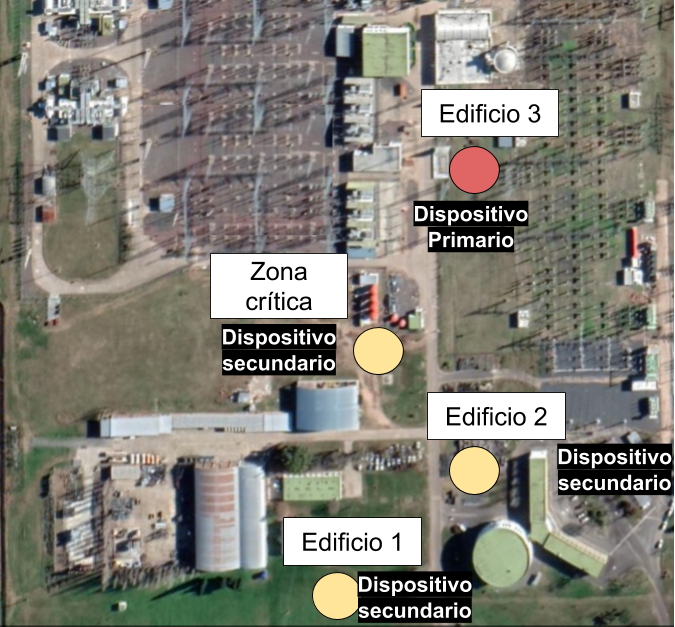
\includegraphics[scale=.4]{./Figures/Capitulo3/Fig_A3.png}
	\caption{Ejemplo de sistema de detección de incendio complejo.}
	\label{fig:figura_a3}
\end{figure}

\section{Criterios de diseño}

El sistema corresponde al primero de una serie de proyectos que tienen como objetivo la generación de alternativas de monitoreo de sistemas de detección de incendio. En esta etapa el objetivo propuesto es reportar al usuario únicamente el estado de la instalación, pero en futuros proyectos se desea alcanzar un mayor nivel de detalle. A continuación se describen los criterios considerados para la selección de los componentes:

Escalabilidad: el sistema debe contar con los recursos necesarios para la integración de nuevas funcionalidades o servicios.

Robustez: una característica que se desea proporcionar a los sistemas es la posibilidad de tener formas alternativas de trabajo ante eventos de falla.

Recuperabilidad: el mantenimiento de equipos de detección de incendio suele realizarse de forma mensual, por lo que el sistema debe estar en capacidad de restituirse de forma automática en caso de fallas, para evitar visitas adicionales por fallas del dispositivo de monitoreo.

Documentación adecuada:  el sistema debe desarrollarse a partir de plataformas con documentación detallada y de fácil acceso.

Disponibilidad en el mercado argentino: los sistemas deberán estar compuestos por elementos que puedan ser adquiridos en el mercado local.

\subsubsection{Criterios fundamentales}

Es de suma importancia respetar dos criterios principales:
\begin{itemize}
\item La no afectación la secuencia de accionamiento de la central de forma remota. 
\item El sistema de monitoreo no debe utilizarse como un dispositivo de detección de incendio.
\end{itemize}

El esquema de conexión entre el dispositivo de monitoreo y la central de alarma de incendio recomendado
se muestra en la figura \ref{fig:figura_b3}.

\begin{figure}[]
	\centering
	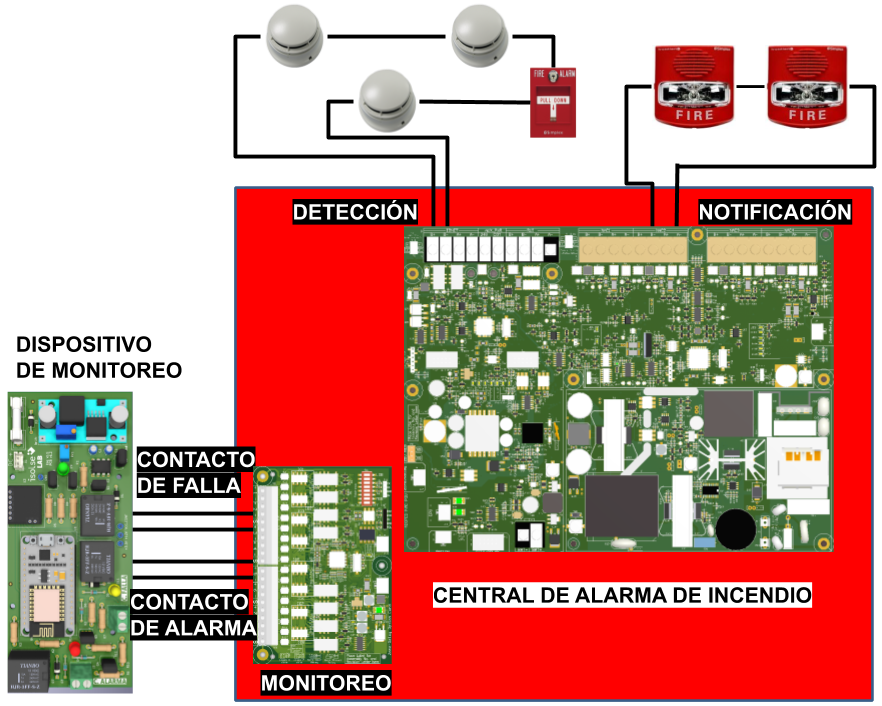
\includegraphics[scale=.35]{./Figures/Capitulo3/Fig_B3.png}
	\caption{Esquema de conexión entre dispositivo de monitoreo y central de alarma de incendio.}
	\label{fig:figura_b3}
\end{figure}

\section{Arquitectura general del sistema}

En esta fase se procede a describir los elementos que componen el sistema de monitoreo, su funcionamiento y la interconexión entre cada componente.


\subsection{Dispositivo primario} 

Un sistema de monitoreo compuesto por este dispositivo únicamente cuenta con los recursos necesarios para el monitoreo de un sistema de detección de alarma base, compuesto por una única central de alarma de incendio a monitorear. El dispositivo implementa un monitoreo periodico a los contactos de alarma y falla para determinar el estado del equipo local; el siguiente paso es facilitar esta información al usuario  para lo que hace uso de tres recursos de notificación:
\begin{itemize}
\item Leds de indicación de estado.
\item Interfaz web para notificación local, por medio de la plataforma Node-RED.
\item Servidor web firebase.
\end{itemize}

A pesar de ser un dispositivo para el monitoreo de un sistema de detección de alarma base este dispositivo considera la posibilidad de un sistema de detección complejo, por lo que dispone de un módulo específico para la gestión de comunicación inalámbrica que permite al sistema comunicarse con diferentes dispositivos de monitoreo secundarios.

El dispositivo primario procesa el estado local y los estados remotos para generar un diagnóstico del sistema de detección en general, de esta forma en caso de no existir vinculación entre los equipos de detección de alarma el sistema es capaz de establecer el estado correcto de la instalación en su totalidad.

El diseño general del dispositivo primario se puede observar en la figura \ref{fig:figura_c3}.

\begin{figure}[h]
	\centering
	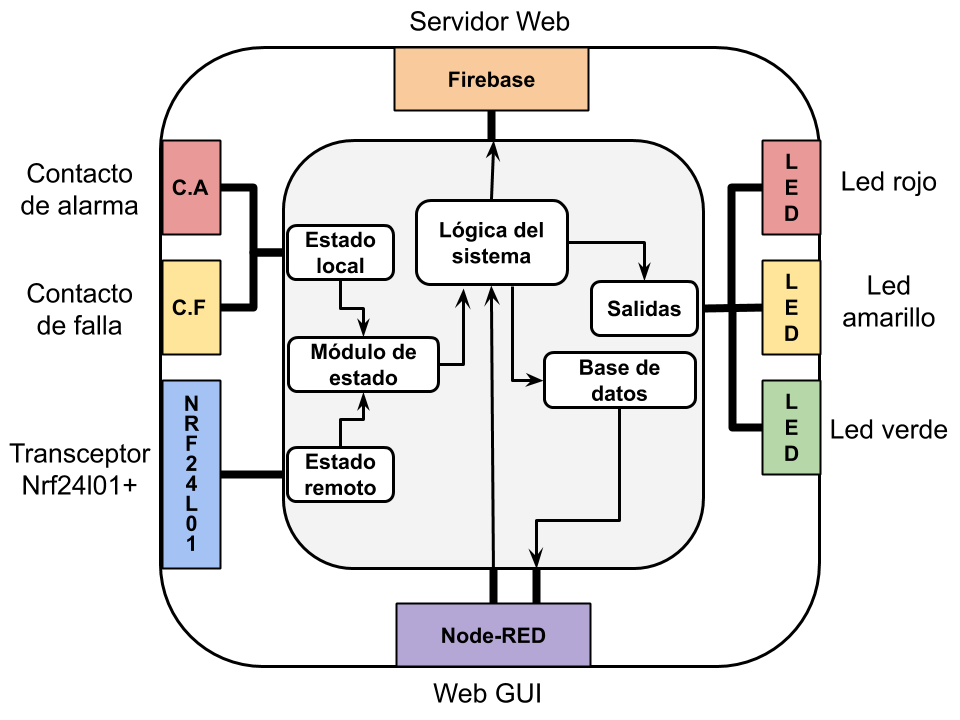
\includegraphics[scale=.4]{./Figures/Capitulo3/Fig_C3.png}
	\caption{Arquitectura del dispositivo primario.}
	\label{fig:figura_c3}
\end{figure}

\subsection{Dispositivo secundario}

Este dispositivo realiza el  monitoreo del contacto de alarma y del contacto de falla, y cuenta con módulo destinado a la gestión de la transmisión de información mediante comunicación inalámbrica. El sistema presenta la información al usuario de acuerdo a la condición existente en la instalación: rojo indica alarma, amarillo indica falla y verde, condición normal.


Incluir en el diseño un dispositivo secundario permite agregar un equipo adicional a monitorear, y además incrementa el alcance de la comunicación inalámbrica, ya que cada nodo actúa como nodo-repetidor. En la figura \ref{fig:figura_d3} se observa el diseño general del dispositivo secundario.


\begin{figure}[]
	\centering
	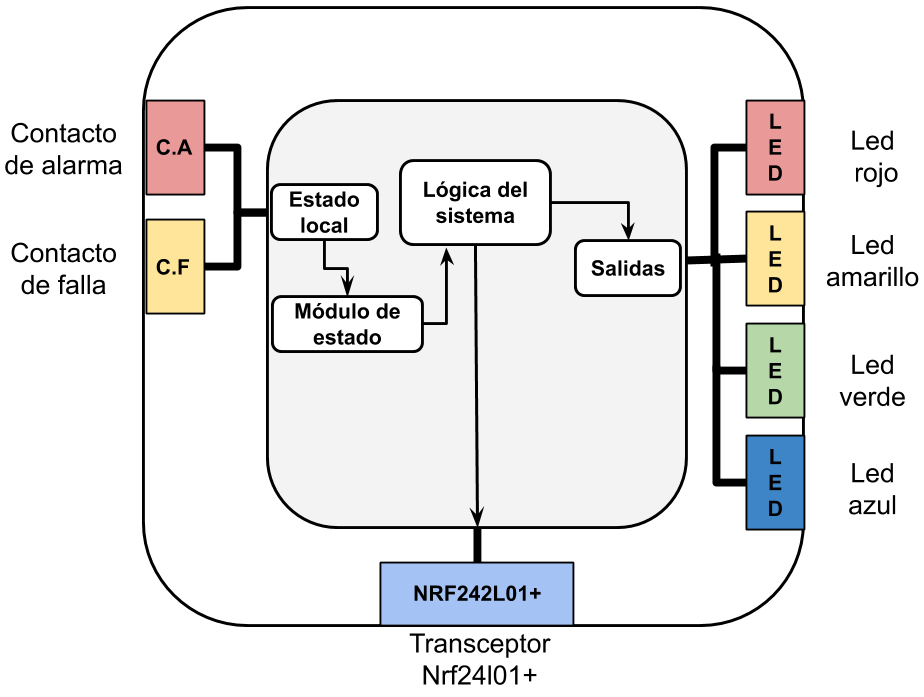
\includegraphics[scale=.4]{./Figures/Capitulo3/Fig_D3.png}
	\caption{Arquitectura del dispositivo secundario.}
	\label{fig:figura_d3}
\end{figure} 

\subsection{Aplicación en sistemas de detección complejos}

Una instalación como la descrita en la figura \ref{fig:figura_a3}, compuesta por tres edificios y una zona crítica, puede ser monitoreada con una arquitectura como la dispuesta en la figura \ref{fig:figura_e3}, donde se puede observar las interfaces entre los elementos del sistema.

\begin{figure}[]
	\centering
	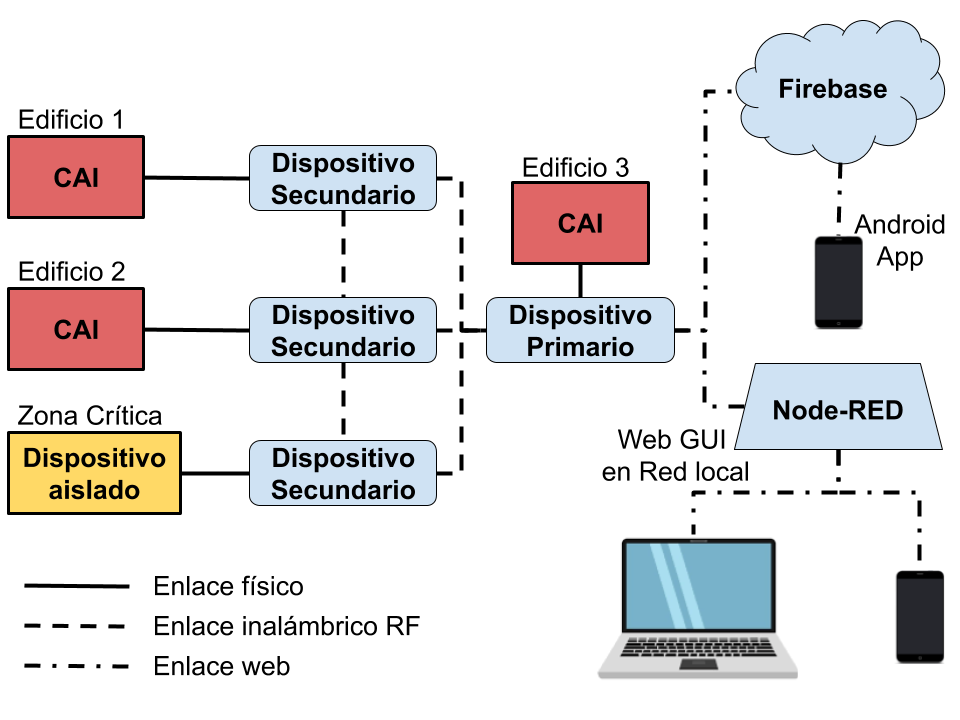
\includegraphics[scale=.4]{./Figures/Capitulo3/Fig_E3.png}
	\caption{Arquitectura general del dispositivo de monitoreo remoto.}
	\label{fig:figura_e3}
\end{figure} 

\newpage

\section{Hardware}

Esta sección describe el  diseño del hardware utilizado para los dispositivos primario y secundario, sus características, módulos internos y la relación entre ellos.

\subsection{Hardware del dispositivo primario}

Los esquemáticos empleados para la implementación del hardware del dispositivo primario se pueden observar en las figuras \ref{fig:figura_f3}, \ref{fig:figura_g3} y \ref{fig:figura_h3}. El diseño fue concretado como un poncho para la Raspberry Pi, compuesto por los módulos detallados a continuación:

\subsubsection{Módulo de monitoreo de contacto seco}

El diseño de este módulo hace uso del contacto normal abierto del dispositivo a monitorear para la indicación de alarma o falla en el sistema. La indicación correspondiente se hace a través del accionamiento de un relé interno que modifica el estado del circuito asociado.
La figura \ref{fig:figura_f3} muestra el esquema del módulo de monitoreo de contacto seco.

\begin{figure}[]
	\centering
	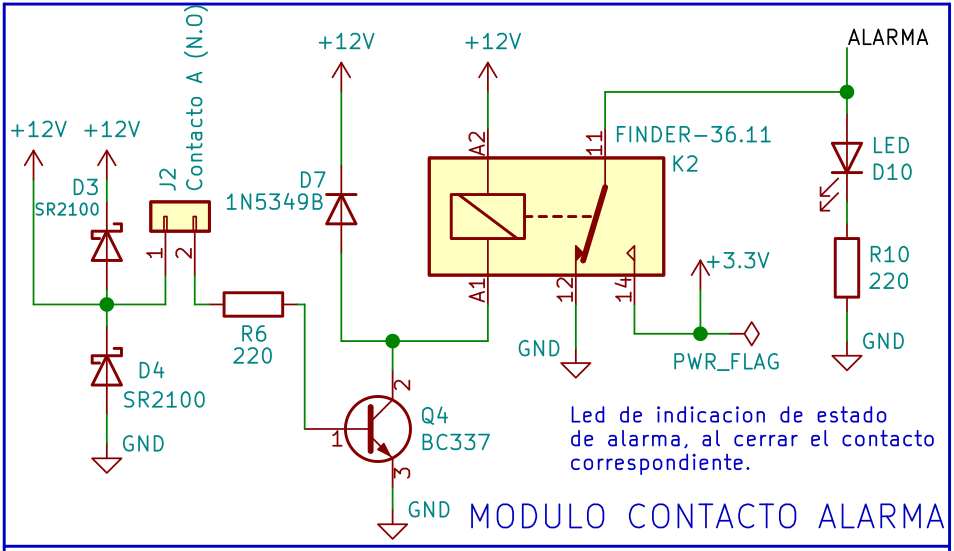
\includegraphics[scale=.35]{./Figures/Capitulo3/Fig_F3.png}
	\caption{Módulo de monitoreo de contacto seco de alarma.}
	\label{fig:figura_f3}
\end{figure} 

El diseño considera la posibilidad de ocurrencia de un error de conexión, para lo cual se incluyó una etapa de protección, que se encarga de mantener la tensión dentro de los rangos de trabajo del dispositivo [0 - 12] VDC.

\subsubsection{Módulo de comunicación nrf24l01+}

La conexión del módulo transceptor nrf24l01+ se hace siguiendo el esquema recomendado [bibliografía], como puede observarse en la figura \ref{fig:figura_g3}, consiste en una conexión directa con el dispositivo y en utilizar la fuente de 3,3 VDC del dispositivo primaria para energizarlo.  

\begin{figure}[]
	\centering
	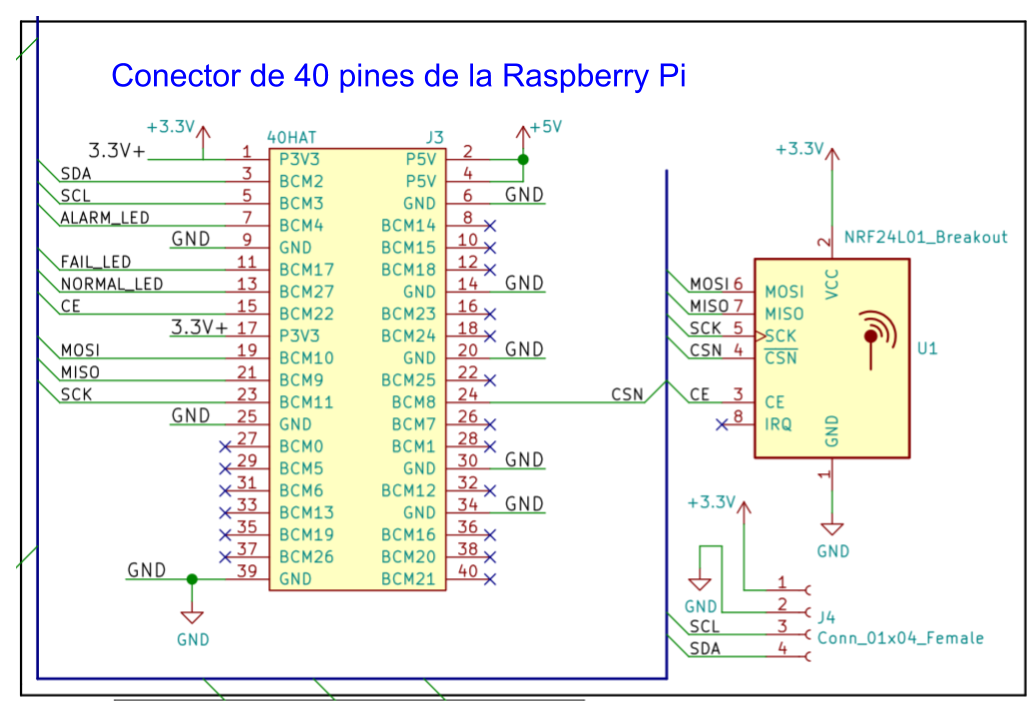
\includegraphics[scale=.35]{./Figures/Capitulo3/Fig_G3.png}
	\caption{Módulo de comunicación inalámbrica.}
	\label{fig:figura_g3}
\end{figure} 

\subsubsection{Módulo de notificación visual}

El módulo sigue lo establecido por los requerimientos  2.3.9 y permite al dispositivo reportar el estado del sistema a monitorear de forma local, sin necesidad de dispositivos adicionales. En la figura \ref{fig:figura_h3} se presentan las conexiones y pines utilizados por el sistema.

\begin{figure}[]
	\centering
	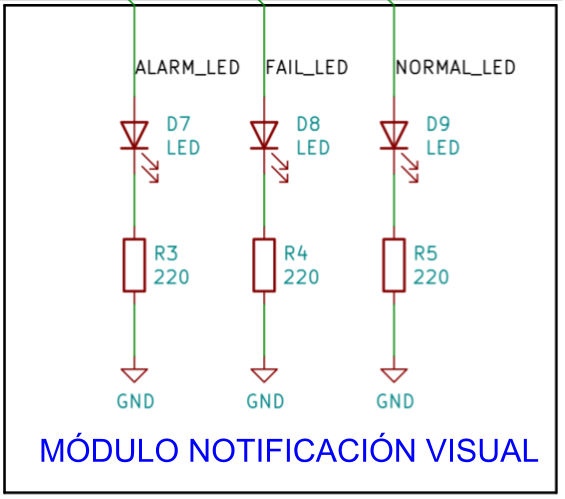
\includegraphics[scale=.25]{./Figures/Capitulo3/Fig_H3.png}
	\caption{Módulo de notificación visual.}
	\label{fig:figura_h3}
\end{figure} 


\subsection{Hardware del dispositivo secundario}

El diseño del sistema puede observarse en las figuras \ref{fig:figura_j3},\ref{fig:figura_k3},\ref{fig:figura_l3}, se reutiliza el diseño de la figura \ref{fig:figura_f3} para el monitoreo de contactos y se añaden al sistema los módulos descritos a continuación.

\subsubsection{Módulo de comunicación nrf24l01+ con amplificador de potencia}

El dispositivo secundario utiliza un módulo nrf24l01+ con un amplificador de potencia, por lo que a diferencia del dispositivo primario emplea un adaptador para la conexión del módulo que garantiza una tensión de alimentación estable. El esquema de conexión se detalla en la figura \ref{fig:figura_j3}.

\begin{figure}[]
	\centering
	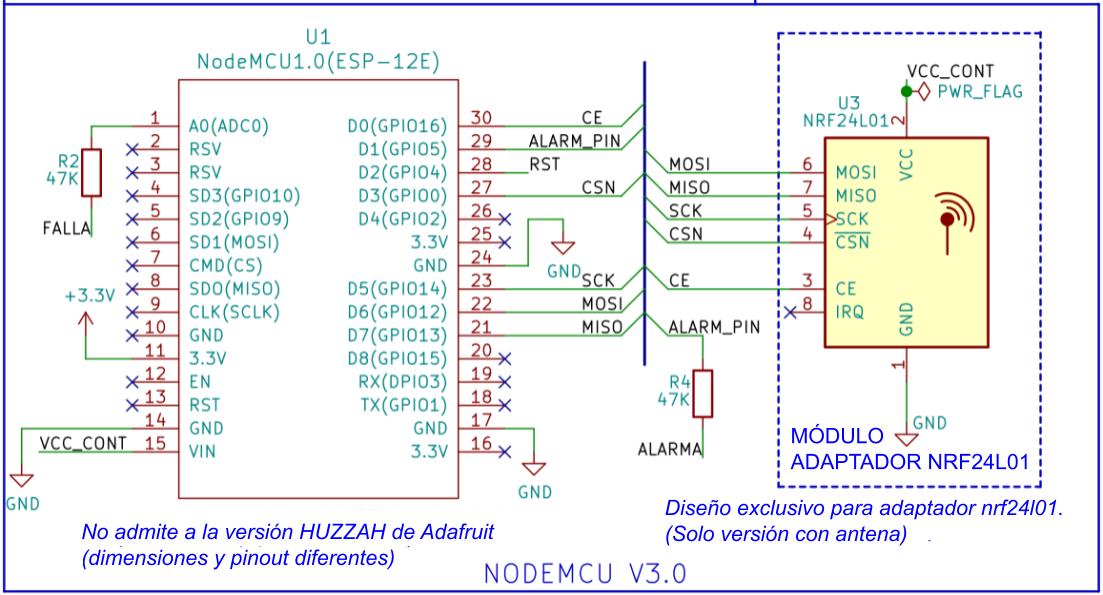
\includegraphics[scale=.3]{./Figures/Capitulo3/Fig_J3.png}
	\caption{Módulo de comunicación inalámbrica de largo alcance.}
	\label{fig:figura_j3}
\end{figure} 


\subsubsection{Módulo de notificación visual}

Debido a restricciones del dispositivo con respecto al número de GPIO disponible el sistema no implementa una conexión directa con el led de notificación de estado normal. En la figura \ref{fig:figura_k3} se puede verificar que el encendido del led indicador del estado normal se realiza a través de hardware ante la ausencia de señales de falla o alarma.

\begin{figure}[]
	\centering
	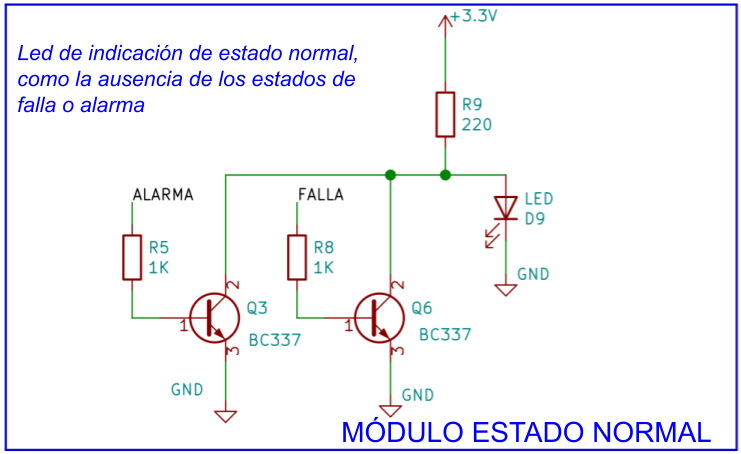
\includegraphics[scale=.35]{./Figures/Capitulo3/Fig_K3.png}
	\caption{Módulo de notificación visual.}
	\label{fig:figura_k3}
\end{figure} 


\subsubsection{Módulo de alimentación}

La alimentación del dispositivo se obtiene a partir del módulo LM2596S-123-3000, un regulador de tensión continua regulable, configurado a 12 vdc. La figura \ref{fig:figura_l3} exhibe al módulo de alimentación y el diseño de una etapa de protección ante casos de conexión con polaridad inversa.

\begin{figure}[]
	\centering
	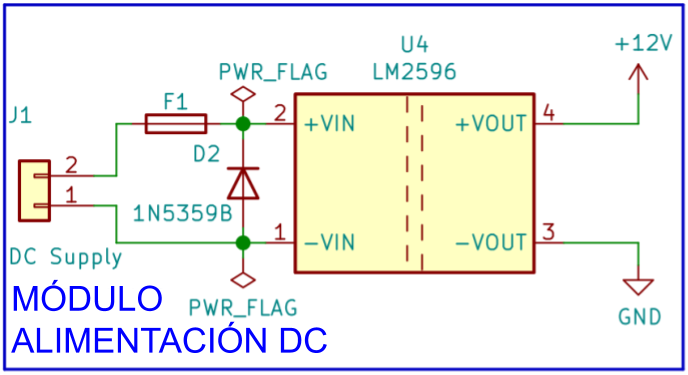
\includegraphics[scale=.3]{./Figures/Capitulo3/Fig_L3.png}
	\caption{Módulo de notificación visual.}
	\label{fig:figura_l3}
\end{figure} 


\section{Software}

Esta sección describe  el funcionamiento de los módulos lógicos más importantes de cada dispositivo; se resaltan las consideraciones y flujo de acciones que rigen en cada caso.

\subsection{Dispositivo primario}

El dispositivo primario funciona a partir del diagrama de flujo de la figura \ref{fig:figura_disp_prim}, para ello utiliza los recursos del sistema operativo Raspbian para la generación de un programa multi hilos, lo que permite desarrollar un sistema escalable y segmentado organizado de la siguiente forma: 

\begin{figure}[]
	\centering
	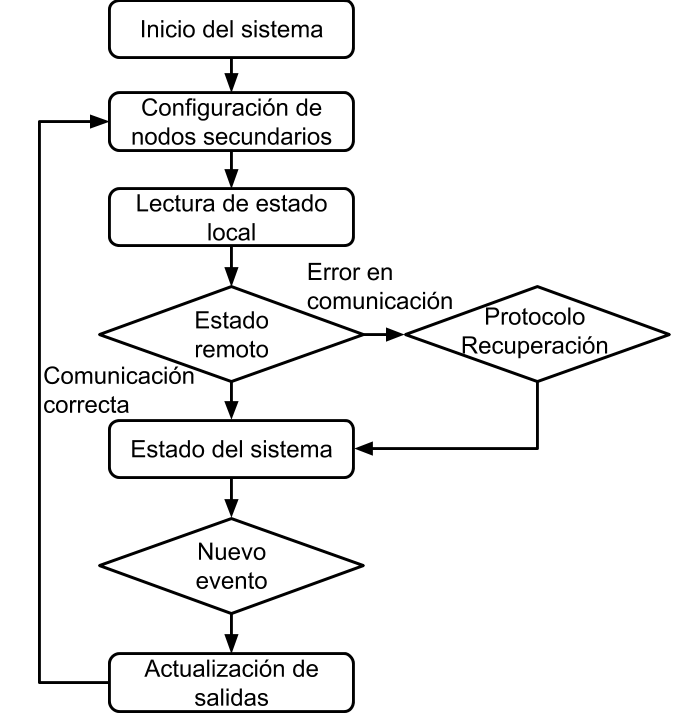
\includegraphics[scale=.3]{./Figures/Capitulo3/Fig_Fl_Pri.png}
	\caption{Diagrama de flujo del dispositivo primario.}
	\label{fig:figura_disp_prim}
\end{figure} 

\begin{itemize}
\item Tareas de actualización: aquellas funcionalidades con mayor prioridad y de ejecución frecuente generan la información que utilizarán las tareas de control para determinar las acciones correspondientes.
\item Tareas de control: este segmento agrupa aquellas funciones dependientes del estado actual y la información obtenida de las tareas de actualización, modifican el estado actual y las salidas del sistema. 
\item Tareas de notificación periódica: el sistema genera una validación cada segundo en la que verifica el estado actual tanto del sistema de detección de incendio, como el del subsistema de comunicación inalámbrica para luego proceder a actualizar los archivos de registro bases de datos del sistema para la actualización de las interfaces de notificación al usuario.
\item Tareas de mantenimiento: las tareas de control tienen la potestad de activar tareas específicas para intentar reponer fallas en el sistema asociadas a la comunicación inalámbrica. Estas funcionalidades otorgan al programa un protocolo de recuperación que permite reiniciar la interfaz de comunicación con el módulo transceptor nrf24l01.
\end{itemize}

La organización del sistema en segmentos de tareas donde cada una se ejecuta con un objetivo específico proporciona una estructura al software que estandariza el proceso de inclusión de nuevas funcionalidades.  A continuación se describe el flujo de los segmentos de código ejecutados por el dispositivo primario:

\subsubsection{Módulo de estado}

El sistema tiene cuatro posibles transiciones:
\begin{itemize}
\item Alarma y falla.
\item Alarma.
\item Falla.
\item Normal.  
\end{itemize}

Este módulo se encarga de definir cuál de estas transiciones debe ser ejecutada. Su funcionamiento requiere evaluar tanto el estado del dispositivo local monitoreado como el cada uno de los estados remotos provenientes de los dispositivos secundarios.

El enfoque utilizado se puede analizar en el diagrama de flujo de la figura \ref{fig:figura_n3}. El sistema funciona a partir de ventanas de tiempo de 200 ms, durante los cuales se registran los siguientes datos de cada mensaje recibido: código de identificación del remitente, código asociado al estado del sistema monitoreado y estado del dispositivo. Los primeros dos elementos provienen del dispositivo secundario que estableció la comunicación, sin embargo el tercer elemento es impuesto por el dispositivo primario, cada vez que el sistema recibe un código establece el estado del nodo como activo. De esta forma se indica qué dispositivos se encuentran comunicándose correctamente.

\begin{figure}[]
	\centering
	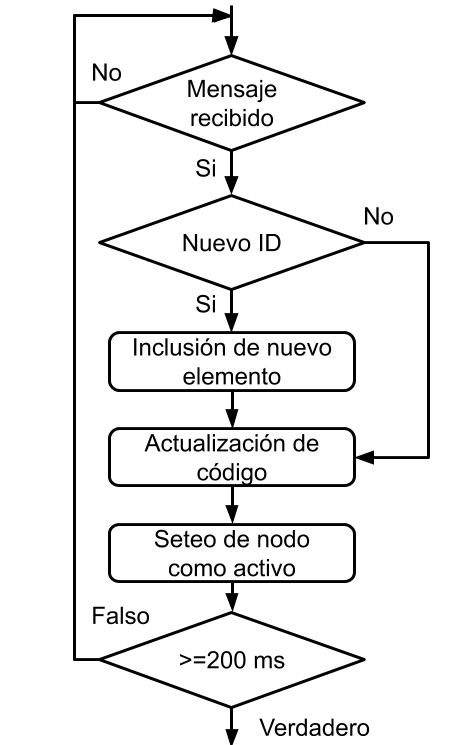
\includegraphics[scale=.35]{./Figures/Capitulo3/Fig_N3.png}
	\caption{Diagrama de flujo del módulo de estado.}
	\label{fig:figura_n3}
\end{figure}  


\subsubsection{Protocolo de recuperación}

Con la intención de generar un sistema que requiera del menor mantenimiento correctivo posible se implementa un protocolo ante fallas de comunicación inalámbrica. El sistema funciona según lo descrito en la figura \ref{fig:figura_o3}. Este busca busca tomar ventaja de las características del módulo nrf24l01 para establecer un sistema de comunicación robusto con la capacidad de recuperarse de forma automática.

\begin{figure}[]
	\centering
	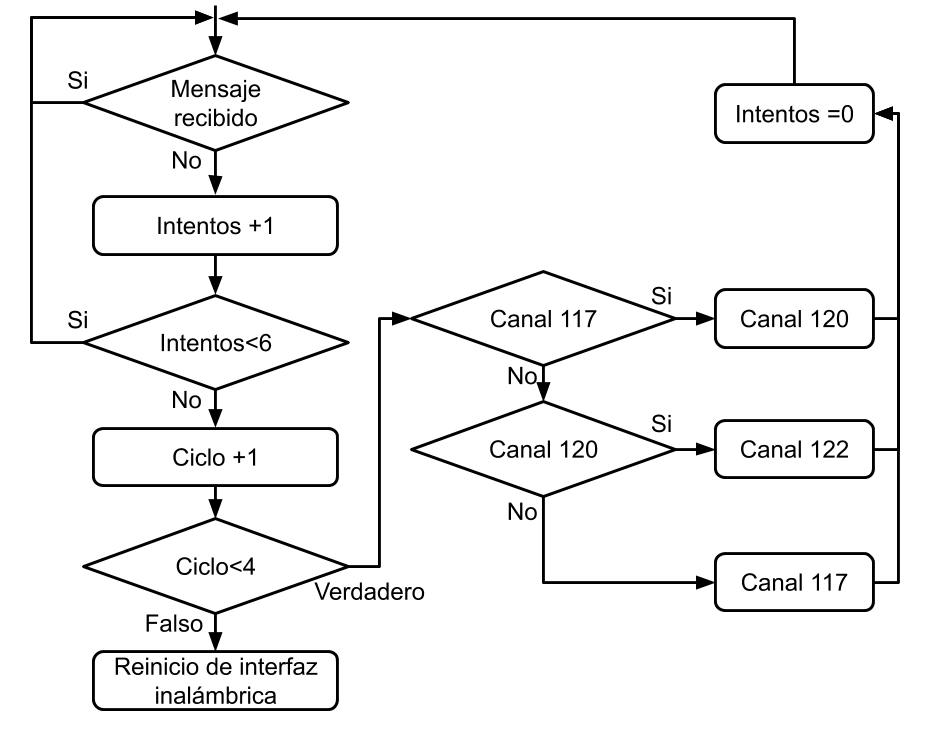
\includegraphics[scale=.35]{./Figures/Capitulo3/Fig_O3.png}
	\caption{Diagrama de flujo del protocolo de recuperación.}
	\label{fig:figura_o3}
\end{figure}  

Este módulo clasifica el estado de la comunicación en cuatro posibles estados: ``sin problemas'',  ``incompleto'',  ``saltando'' y  ``en reparación'', cada uno hace referencia a una etapa del protocolo de recuperación:  

\begin{itemize}
\item Sin problemas: el sistema hace una serie de intentos a una determinada frecuencia; si logra establecer la comunicación con la cantidad de dispositivos secundarios especificada no se presentan fallas de comunicación y se concluye que el sistema funciona correctamente.
\item Saltando: en caso de que el sistema no reciba información de ninguno de los dispositivos secundarios procede a realizar una serie de intentos en la misma frecuencia, hasta alcanzar un número de cinco intentos. Si la falla se mantiene procede a realizar un salto de frecuencia, y reiniciar el conteo de intentos a cero. Este salto se puede realizar un máximo de dos veces por lo que al alcanzar el tercer salto se procederá a la siguiente etapa. 
\item Reparación: el ciclo descrito para el estado ``saltando'' ahora se contabiliza. Si este ciclo de intentos se realiza tres veces consecutivas y no se logra establecer comunicación con ninguno de los dispositivos el sistema procederá a realizar un reinicio de la interfaz con el nodo transceptor nrf24l01+, se eliminan los registros asociados y comienza el ciclo nuevamente.
\item Incompleto: el protocolo de recuperación existe únicamente para casos en los que no se pueda establecer la comunicación con ninguno de los dispositivos secundarios. Si por el contrario al menos un dispositivo secundario se comunica correctamente el protocolo no es ejecutado ya que en esa frecuencia existe un dispositivo. Dependerá del resto de dispositivos secundarios modificar su canal de transmisión para sincronizarse con el dispositivo primario.  
\end{itemize}

\subsubsection{Lógica del sistema}

El dispositivo primario contiene la lógica de las transiciones posibles para el sistema, que se puede analizar a partir del esquema de la figura \ref{fig:figura_p3} que ilustra cómo deben ser los cambios de estado a partir de las condiciones de transición presentes. La figura introduce los  ``estados previos'' que permiten generar acciones antes de la activación de un estado específico y más importante aún, funcionan como un elemento de validación, ya que hacen necesario que la transición entre estados principales (alarma y falla, alarma, normal y falla) se realice únicamente ante dos transiciones del mismo tipo.

\begin{figure}[]
	\centering
	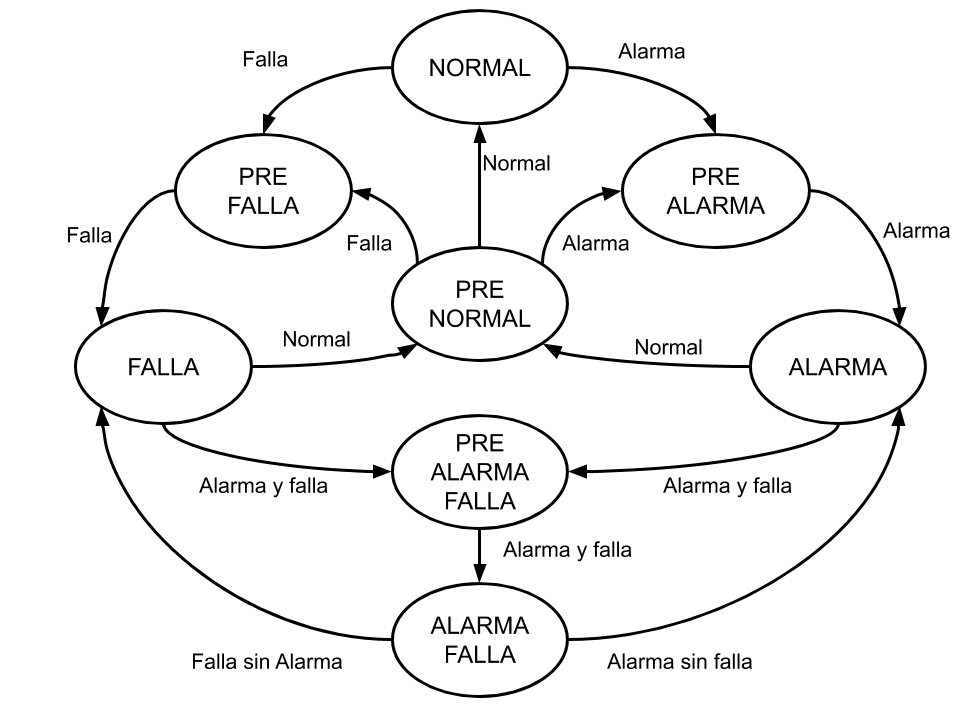
\includegraphics[scale=.35]{./Figures/Capitulo3/Fig_P3.png}
	\caption{Diagrama de flujo de la lógica del sistema.}
	\label{fig:figura_p3}
\end{figure}  

El segmento de código \ref{cod:vControl} se alimenta a partir de la información generada por el módulo de estado. Realiza un análisis con el objetivo de determinar la transición adecuada y la cantidad de dispositivos secundarios activos. Esta información es procesada junto con el estado actual para establecer el nuevo estado y las acciones correspondientes a ejecutar.

\begin{lstlisting}[label=cod:vControl,caption=Pseudocódigo de  de mensajes inalámbricos.]  % Start your code-block

int Comm_Code(RF_List_t* RF_List,Nodes_Database_t* Data_RF_List)
{
	int Final_Code;
	bool Alarm=0;
	bool Fail=0;
	int i;
	int counter=0;
	RF_Device_t * Mem_Block;
		
	Data_RF_List->Counter=0;
	
	
//	- Ciclo de verificacion de estados  

	for(i=0;i<RF_List->counter;i++)
	{	
		Mem_Block=RF_List->RF_Devices[i];
		Update_Node_Data(Mem_Block[0],Data_RF_List,i);

		if(Mem_Block[0].updated)	// El nodo fue actualizado?
		{
			counter++;
			Mem_Block[0].updated=0;
			
			if(ALARM_FAIL_CODE==Mem_Block[0].RF_Code)
			{
				Alarm=1;
				Fail=1;
			}
		
			if(ALARM_CODE==Mem_Block[0].RF_Code)
			{
				Alarm=1;
			}
			
			if(FAIL_CODE==Mem_Block[0].RF_Code)
			{
				Fail=1;
			}
		}
	}
	RF_List->active_nodes = counter; //Registro de cantidad de nodos activos

	if((Alarm)&&(Fail))
	{
		Final_Code = ALARM_FAIL_CODE;
	}else if(Alarm)
	{
		Final_Code = ALARM_CODE;
	}else if(Fail)
	{
		Final_Code = FAIL_CODE;
	}else
	{
		Final_Code = NORMAL_CODE;
	}
	//Si existe al menos una alarma o una falla	el sistema cambia a dicho estado.
	return Final_Code;
}
\end{lstlisting}

% CODIGO!!!!!!!!!!

\subsection{Servicios de interacción con el usuario}

\subsubsection{Interfaz Web}

El software utilizado funciona a partir del monitoreo de cambios recientes en un archivo de registro de eventos, que hace la función de histórico de eventos del sistema. Se valida cada cinco segundos el estado del sistema, y en caso de encontrar diferencias entre el estado anterior y el estado actual, el registro se modifica, lo que provoca una actualización en la plataforma web gestionada por Node-RED.  

La plataforma Node-RED gestiona la interacción con el usuario a nivel local, lo que significa que siempre que el usuario se encuentre conectado a la misma red del sistema de monitoreo de detección de incendio se le otorgará acceso a esta interfaz, que le permitirá configurar del sistema y observar el estado en general. Esta decisión evita la modificación del sistema de detección de incendio de forma remota.         

\subsubsection{Firebase}

La base de datos de Firebase se actualiza a partir del archivo histórico de eventos, de donde se extrae la información más reciente y se carga a partir de un script de Python en el servidor web de Firebase.

Este módulo propone una alternativa para el monitoreo del sistema de forma remota desde cualquier punto con conexión a  Internet. La plataforma brinda un servicio de \textit{realtime database}, que posee integraciones con diferentes elementos como páginas web, aplicaciones Android o IOS. El módulo Firebase no provee al usuario la posibilidad de configurar ningún parámetro. En otras palabras funciona únicamente para monitorear el estado del sistema de forma remota.

\subsubsection{Bases de datos}

Una alternativa al archivo de histórico de eventos es el registro de eventos a través del uso de bases de datos con la biblioteca SQLite; el sistema genera las siguientes bases de datos:
\begin{itemize}
\item Histórico de eventos: registro de cualquier tipo de eventos como alarmas, fallas y cambios en el estado de la comunicación inalámbrica.
\item Detalle de comunicación inalámbrica: se recibe información de diferentes nodos, estos datos quedan registrados y son actualizados cada vez que se establece un nuevo estado remoto. Esto hace posible obtener un detalle de cuáles dispositivos se encuentran comunicándose correctamente con el dispositivo primario.    
\end{itemize}

\subsection{Dispositivo secundario}

Es un dispositivo enfocado en la transmisión del estado del dispositivo monitoreado. La figura \ref{fig:figura_disp_fl_sec} expone el diagrama de flujo utilizado por el sistema. Una vez adquirido el estado del sistema a monitorear se procede a transmitirlo al dispositivo primario y en caso de falla se ejecuta el protocolo de recuperación según corresponda.

El software del dispositivo secundario se basa en un sistema operativo cooperativo que distribuye las funcionalidades del sistema en un arreglo de tareas cada una con un enfoque particular, muy similar a la arquitectura utilizada para el dispositivo primario.

\begin{figure}[]
	\centering
	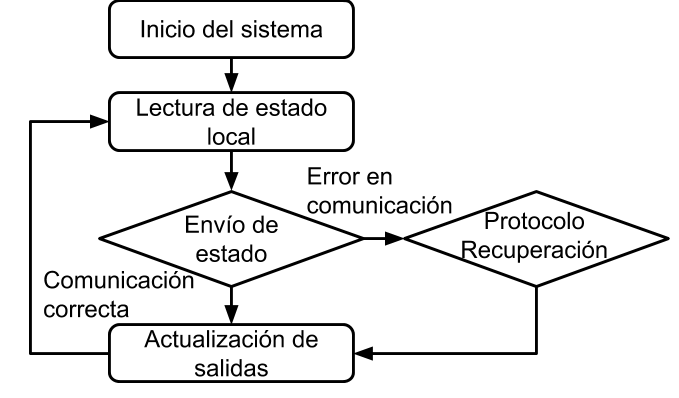
\includegraphics[scale=.35]{./Figures/Capitulo3/Fig_Fl_Sec.png}
	\caption{Diagrama de flujo general del dispositivo secundario.}
	\label{fig:figura_disp_fl_sec}
\end{figure} 
%***********************************************

El dispositivo secundario se resume a una versión del dispositivo primario orientado únicamente a la transmisión del estado actual mediante el módulo nrf24l01.
